\chapter{Pollard-Rho para resolver ECDLP}
Em 1978, Pollard veio com o método Monte-Carlo\footnote{Monte-Carlo é qualquer método de uma classe de métodos estatísticos que se baseiam em amostragens aleatórias massivas para obter resultados númericos, isto é, repetindo sucessivas simulações um elevado número de vezes, para calcular probabilidades de forma heurística.} para resolver o problema do logaritmo discreto. Desde então, o método foi modificado para resolver o ECDLP. Como o algoritmo Pollard-Rho é atualmente o algoritmo mais rápido para resolver o ECDLP, então a segurança do ECC depende da eficiência desse algoritmo. Teoricamente, se o algoritmo Pollard-Rho é capaz de resolver o ECDLP eficientemente e em um tempo relativamente curto, então o criptossistema estará inseguro. \cite{Mandy:2007}

A estratégia do algoritmo é produzir uma sequência de termos gerados randomicamente $(R_k, a_k, b_k)$, onde \(R_k\) é um ponto na curva \(E\) e \(a_k\)  e \(b_k\) estão em $\mathbb{F}_p$ sobre a qual a curva elíptica \(E\) está definida. Como $E(\mathbb{F}_p)$ é um grupo finito, a sequência eventualmente irá torna-se periódica e voltará para um termo anterior da sequência. Usa-se essa periodicidade para resolver ECDLP. Como nem sempre a sequência volta para o primeiro termo, um diagrama da sequência parecerá com a letra Grega \(\rho\) (Ver figura \ref{fig:rho}). Por este motivo esse método é chamado de Pollard-Rho. Essa sequência de termos gerados é chamada de ``percurso''.

Seja \(\mu\) o tamanho da calda e \(\lambda\) o tamanho do ciclo. Após um número finito de iterações, obtêm-se os termos $R_k = R_{k+\lambda}$, onde $k > \mu$ e $\lambda > 1$. Neste ponto, já deverá ter sido encontrado uma correspondência entre os termos e poderá aplicar matemáticas discretas para resolver os problemas de logaritmo discreto gerado pelos elementos do conjunto finito.

\begin{figure}[h]
\centering
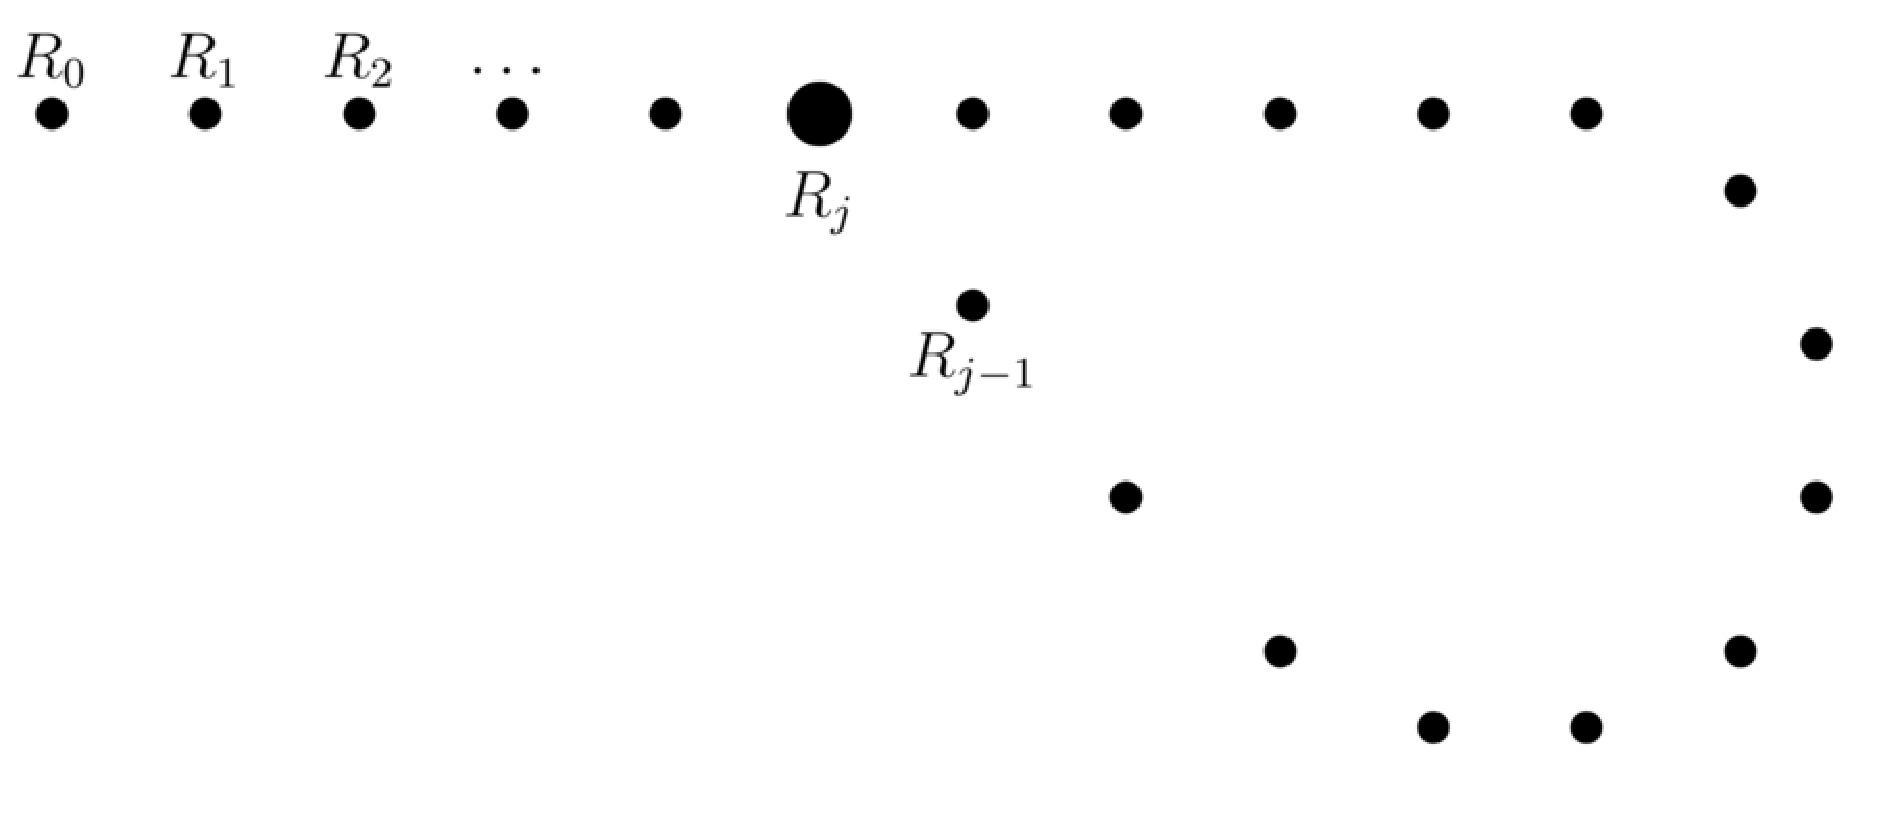
\includegraphics[scale=0.4, bb=0 0 888 376]{figuras/rho.eps}
\caption{Diagrama da sequência produzida pelo algoritmo Pollard-Rho}
\label{fig:rho}
\end{figure}

\section{Algoritmo de Pollard-Rho}
Seja $G = E(\mathbb{F}_p)$, tal que a ordem de $G = n$, e \(P\) e \(Q\) tal que $Q = xP$ em \(G\). O objetivo é calcular \(x\). Segue os passos:

\begin{enumerate}
\item Usando uma função \textit{hash}, \(G\) é particionado em 3 conjuntos $S_1, S_2, S_3$ de aproximadamente do mesmo tamanho, em que $O \notin S_2$.
\item Definir uma função de iteração $f : R \to R$ de um percurso aleatório:

\begin{eqnarray} \label{eq:walk}
R_{k+1} = f(R_k) =
\begin{cases}
Q + R_k, &R_k \in S_1 \\
2R_k, &R_k \in S_2 \\
P + R_k, &R_k \in S_3
\end{cases}
\end{eqnarray}

\item Seja $R_k = a_kP + b_kQ$, e portanto

\begin{eqnarray}
a_{k+1} =
\begin{cases}
a_k, &R_k \in S_1 \\
2a_k \pmod n, &R_k \in S_2 \\
a_k + 1, &R_k \in S_3
\end{cases}
\end{eqnarray}

e

\begin{eqnarray}
b_{k+1} =
\begin{cases}
b_k + 1, &R_k \in S_1 \\
2b_k \pmod n, &R_k \in S_2 \\
b_k, &R_k \in S_3
\end{cases}
\end{eqnarray}

\item Os termos iniciais são: $R_0 = P, a_0 = 1, b_0 = 0$ e os pares gerados $(R_k, R_{2k})$ até encontrar uma correspondência $R_m = R_{2m}$, para qualquer \(m\).

\item Uma vez encontrados, calcule:

\begin{eqnarray*}
R_m = a_mP + b_mQ \\
R_{2_m} = a_{2_m}P + b_{2m}Q
\end{eqnarray*}

\item Com isso, é possível calcular \(x\):

\begin{equation} \label{eq:x}
x = (a_{2m} - a_m)(b_m - b_{2m})^{-1} \pmod n
\end{equation}

\end{enumerate}

Assumindo que o percuso aleatório \ref{eq:walk} definido no algoritmo produz termos aleatórios, então a primeira colisão na sequência é esperada para após $\sqrt{\pi n/2}$ termos. Além disso, o tamanho da calda prevista é de $\mu \approx \sqrt{\pi n/8}$ e o tamanho do ciclo $\lambda \approx \sqrt{\pi n/8}$. \cite{Pollard:1978}

O termo $(b_m - b_{2m})^{-1}$ em \ref{eq:x} somente é possível calcular quando o GCD$(b_m - b_{2m}, n) = 1$, ou seja, quando são coprimos entre si. Caso contrário, o algoritmo não poderá continuar.
